\documentclass[]{article}
\usepackage{lmodern}
\usepackage{amssymb,amsmath}
\usepackage{ifxetex,ifluatex}
\usepackage{fixltx2e} % provides \textsubscript
\ifnum 0\ifxetex 1\fi\ifluatex 1\fi=0 % if pdftex
  \usepackage[T1]{fontenc}
  \usepackage[utf8]{inputenc}
\else % if luatex or xelatex
  \ifxetex
    \usepackage{mathspec}
  \else
    \usepackage{fontspec}
  \fi
  \defaultfontfeatures{Ligatures=TeX,Scale=MatchLowercase}
\fi
% use upquote if available, for straight quotes in verbatim environments
\IfFileExists{upquote.sty}{\usepackage{upquote}}{}
% use microtype if available
\IfFileExists{microtype.sty}{%
\usepackage{microtype}
\UseMicrotypeSet[protrusion]{basicmath} % disable protrusion for tt fonts
}{}
\usepackage[margin=1in]{geometry}
\usepackage{hyperref}
\hypersetup{unicode=true,
            pdftitle={Building Deep Learning Models},
            pdfauthor={Xiaoyong Pan, Jenna Reps, Peter R. Rijnbeek,},
            pdfborder={0 0 0},
            breaklinks=true}
\urlstyle{same}  % don't use monospace font for urls
\usepackage{color}
\usepackage{fancyvrb}
\newcommand{\VerbBar}{|}
\newcommand{\VERB}{\Verb[commandchars=\\\{\}]}
\DefineVerbatimEnvironment{Highlighting}{Verbatim}{commandchars=\\\{\}}
% Add ',fontsize=\small' for more characters per line
\usepackage{framed}
\definecolor{shadecolor}{RGB}{248,248,248}
\newenvironment{Shaded}{\begin{snugshade}}{\end{snugshade}}
\newcommand{\KeywordTok}[1]{\textcolor[rgb]{0.13,0.29,0.53}{\textbf{#1}}}
\newcommand{\DataTypeTok}[1]{\textcolor[rgb]{0.13,0.29,0.53}{#1}}
\newcommand{\DecValTok}[1]{\textcolor[rgb]{0.00,0.00,0.81}{#1}}
\newcommand{\BaseNTok}[1]{\textcolor[rgb]{0.00,0.00,0.81}{#1}}
\newcommand{\FloatTok}[1]{\textcolor[rgb]{0.00,0.00,0.81}{#1}}
\newcommand{\ConstantTok}[1]{\textcolor[rgb]{0.00,0.00,0.00}{#1}}
\newcommand{\CharTok}[1]{\textcolor[rgb]{0.31,0.60,0.02}{#1}}
\newcommand{\SpecialCharTok}[1]{\textcolor[rgb]{0.00,0.00,0.00}{#1}}
\newcommand{\StringTok}[1]{\textcolor[rgb]{0.31,0.60,0.02}{#1}}
\newcommand{\VerbatimStringTok}[1]{\textcolor[rgb]{0.31,0.60,0.02}{#1}}
\newcommand{\SpecialStringTok}[1]{\textcolor[rgb]{0.31,0.60,0.02}{#1}}
\newcommand{\ImportTok}[1]{#1}
\newcommand{\CommentTok}[1]{\textcolor[rgb]{0.56,0.35,0.01}{\textit{#1}}}
\newcommand{\DocumentationTok}[1]{\textcolor[rgb]{0.56,0.35,0.01}{\textbf{\textit{#1}}}}
\newcommand{\AnnotationTok}[1]{\textcolor[rgb]{0.56,0.35,0.01}{\textbf{\textit{#1}}}}
\newcommand{\CommentVarTok}[1]{\textcolor[rgb]{0.56,0.35,0.01}{\textbf{\textit{#1}}}}
\newcommand{\OtherTok}[1]{\textcolor[rgb]{0.56,0.35,0.01}{#1}}
\newcommand{\FunctionTok}[1]{\textcolor[rgb]{0.00,0.00,0.00}{#1}}
\newcommand{\VariableTok}[1]{\textcolor[rgb]{0.00,0.00,0.00}{#1}}
\newcommand{\ControlFlowTok}[1]{\textcolor[rgb]{0.13,0.29,0.53}{\textbf{#1}}}
\newcommand{\OperatorTok}[1]{\textcolor[rgb]{0.81,0.36,0.00}{\textbf{#1}}}
\newcommand{\BuiltInTok}[1]{#1}
\newcommand{\ExtensionTok}[1]{#1}
\newcommand{\PreprocessorTok}[1]{\textcolor[rgb]{0.56,0.35,0.01}{\textit{#1}}}
\newcommand{\AttributeTok}[1]{\textcolor[rgb]{0.77,0.63,0.00}{#1}}
\newcommand{\RegionMarkerTok}[1]{#1}
\newcommand{\InformationTok}[1]{\textcolor[rgb]{0.56,0.35,0.01}{\textbf{\textit{#1}}}}
\newcommand{\WarningTok}[1]{\textcolor[rgb]{0.56,0.35,0.01}{\textbf{\textit{#1}}}}
\newcommand{\AlertTok}[1]{\textcolor[rgb]{0.94,0.16,0.16}{#1}}
\newcommand{\ErrorTok}[1]{\textcolor[rgb]{0.64,0.00,0.00}{\textbf{#1}}}
\newcommand{\NormalTok}[1]{#1}
\usepackage{longtable,booktabs}
\usepackage{graphicx,grffile}
\makeatletter
\def\maxwidth{\ifdim\Gin@nat@width>\linewidth\linewidth\else\Gin@nat@width\fi}
\def\maxheight{\ifdim\Gin@nat@height>\textheight\textheight\else\Gin@nat@height\fi}
\makeatother
% Scale images if necessary, so that they will not overflow the page
% margins by default, and it is still possible to overwrite the defaults
% using explicit options in \includegraphics[width, height, ...]{}
\setkeys{Gin}{width=\maxwidth,height=\maxheight,keepaspectratio}
\IfFileExists{parskip.sty}{%
\usepackage{parskip}
}{% else
\setlength{\parindent}{0pt}
\setlength{\parskip}{6pt plus 2pt minus 1pt}
}
\setlength{\emergencystretch}{3em}  % prevent overfull lines
\providecommand{\tightlist}{%
  \setlength{\itemsep}{0pt}\setlength{\parskip}{0pt}}
\setcounter{secnumdepth}{5}
% Redefines (sub)paragraphs to behave more like sections
\ifx\paragraph\undefined\else
\let\oldparagraph\paragraph
\renewcommand{\paragraph}[1]{\oldparagraph{#1}\mbox{}}
\fi
\ifx\subparagraph\undefined\else
\let\oldsubparagraph\subparagraph
\renewcommand{\subparagraph}[1]{\oldsubparagraph{#1}\mbox{}}
\fi

%%% Use protect on footnotes to avoid problems with footnotes in titles
\let\rmarkdownfootnote\footnote%
\def\footnote{\protect\rmarkdownfootnote}

%%% Change title format to be more compact
\usepackage{titling}

% Create subtitle command for use in maketitle
\newcommand{\subtitle}[1]{
  \posttitle{
    \begin{center}\large#1\end{center}
    }
}

\setlength{\droptitle}{-2em}

  \title{Building Deep Learning Models}
    \pretitle{\vspace{\droptitle}\centering\huge}
  \posttitle{\par}
    \author{Xiaoyong Pan, Jenna Reps, Peter R. Rijnbeek,}
    \preauthor{\centering\large\emph}
  \postauthor{\par}
      \predate{\centering\large\emph}
  \postdate{\par}
    \date{2018-09-09}

\usepackage{fancyhdr}
\pagestyle{fancy}
\fancyhead{}
\fancyhead[CO,CE]{Building Deep Learning Models}
\fancyfoot[CO,CE]{PatientLevelPrediction Package Version 2.0.5}
\fancyfoot[LE,RO]{\thepage}
\renewcommand{\headrulewidth}{0.4pt}
\renewcommand{\footrulewidth}{0.4pt}

\begin{document}
\maketitle

{
\setcounter{tocdepth}{2}
\tableofcontents
}
\section{Introduction}\label{introduction}

Electronic Health Records data is high dimensional, heterogeneous, and
sparse, which makes predictive modelling a challenge. In the early days,
the machine learning community mainly focused on algorithm development,
currently there is a shift to more powerful feature engineering. Deep
learning models are widely used to automatically learn high-level
feature representations from the data, and have achieved remarkable
results in image processing, speech recognition and computational
biology. Recently, interesting results have been shown in healthcare
applications using EHR data.

This vignette describes how you can use the Observational Health Data
Sciences and Informatics (OHDSI)
\href{http://github.com/OHDSI/PatientLevelPrediction}{\texttt{PatientLevelPrediction}}
package to build deep learning models. This vignette assumes you have
read and are comfortable with building patient level prediction models
as described in the
\href{https://github.com/OHDSI/PatientLevelPrediction/blob/master/inst/doc/BuildingPredictiveModels.pdf}{\texttt{BuildingPredictiveModels}
vignette}. Furthermore, this vignette assumes you are familiar with Deep
Learning methods.

\section{Background}\label{background}

Deep learning models are build by stacking often a large number of
neural network layers that perform feature engineering steps, e.g
embedding, and are collapsed in a final softmax layer (basically a
logistic regression layer). These algorithms need a lot of data to
converge to a good representation, but currently the sizes of the EHR
databases are growing fast which would make Deep Learning an interesting
approach to test within the OHDSI Patient-Level Prediction Framework.
For relatively small Target and Outcome cohorts, Deep Learning is most
probaby not the best choice.

Multiple Deep Learning backends have been developed, e.g.~Tensorflow,
PyTorch, Keras etc. In the package we have implemented interaction with
Keras and PyTorch but we invite the community to add other backends.

Many network topologies have recently been proposed and we have
implemented a number of them, however, this list will grow in the near
future. It is important to understand that some of these topologies
require a 2D data matrix, i.e.
\textbar{}patient\textbar{}x\textbar{}feature\textbar{}, and others use
a 3D data matrix
\textbar{}patient\textbar{}x\textbar{}feature\textbar{}X\textbar{}time\textbar{}.
The FeatureExtraction Package has been extended to enable the extraction
of both data formats as will be described with examples below.

Training Deep Learning Models is computationally intensive, our
implementation therefore supports both GPU and CPU. It will
automatically check whether there is GPU or not in your computer. A GPU
is highly recommended for Deep Learning!

\section{Non-Temporal topologies}\label{non-temporal-topologies}

We implement the following non-temporal (2D data matrix) topologies
using Pytorch:

\begin{verbatim}
1) Logistics regression (LRTorch)
   A simple softmax layer with l2 regularisation

2) Feedforward network (MLPTorch) 
   Supports multilayer perceptron (mlp_type = MLP) and 
   Self-Normalizing Neural Networks (mlp_type = SNN)
   Reference: https://arxiv.org/abs/1706.02515
\end{verbatim}

For the above two methods, we implemented support for a stacked
autoencoder and a variational autoencoder to reduce the feature
dimension as a first step. These autoencoders learn efficient data
codings in an unsupervised manner by stacking multiple layers in a
neural network.

Table 1: Non-Temporal Deep Learning Models Hyper-Parameters

\begin{longtable}[]{@{}lll@{}}
\toprule
\begin{minipage}[b]{0.11\columnwidth}\raggedright\strut
Name\strut
\end{minipage} & \begin{minipage}[b]{0.34\columnwidth}\raggedright\strut
Description\strut
\end{minipage} & \begin{minipage}[b]{0.46\columnwidth}\raggedright\strut
Hyperparameters\strut
\end{minipage}\tabularnewline
\midrule
\endhead
\begin{minipage}[t]{0.11\columnwidth}\raggedright\strut
LRTorch\strut
\end{minipage} & \begin{minipage}[t]{0.34\columnwidth}\raggedright\strut
Logistic Regression Model\strut
\end{minipage} & \begin{minipage}[t]{0.46\columnwidth}\raggedright\strut
w\_decay (l2 regularisation), epochs (number of epochs), class\_weight
(0 = inverse ratio between number of positive and negative examples, -1
= focal loss (\url{https://arxiv.org/abs/1708.02002}), or other),
autoencoder (apply stacked autoencoder?, vae (apply variational
autoencoder)\strut
\end{minipage}\tabularnewline
\begin{minipage}[t]{0.11\columnwidth}\raggedright\strut
MLPTorch\strut
\end{minipage} & \begin{minipage}[t]{0.34\columnwidth}\raggedright\strut
Multi-Layer Perceptron Model\strut
\end{minipage} & \begin{minipage}[t]{0.46\columnwidth}\raggedright\strut
mlp\_type (MLP = default, SNN = self-normalizing neural network), size
(number of hidden nodes), w\_decay (l2 regularisation), epochs (number
of epochs), class\_weight(0 = inverse ratio between number of positive
and negative examples, -1 = focal loss, or other), autoencoder (apply
stacked autoencoder), vae (apply variational autoencoder?)\strut
\end{minipage}\tabularnewline
\bottomrule
\end{longtable}

\subsection{Example}\label{example}

The approach for logistic regression (LRTorch) and the Multi-Layer
Perceptron (MLPTorch) is identical. Here we will take LRTorch as an
example.

You need to generate a \texttt{population} and \texttt{plpData} object
as described in more detail in
\href{https://github.com/OHDSI/PatientLevelPrediction/blob/master/inst/doc/BuildingPredictiveModels.pdf}{\texttt{BuildingPredictiveModels}
vignette}.

Alternatively, you can make use of the data simulator. The following
code snippet creates a population of 12000 patients.

\begin{Shaded}
\begin{Highlighting}[]
\KeywordTok{set.seed}\NormalTok{(}\DecValTok{1234}\NormalTok{)}
\KeywordTok{data}\NormalTok{(plpDataSimulationProfile)}
\NormalTok{sampleSize <-}\StringTok{ }\DecValTok{12000}
\NormalTok{plpData <-}\StringTok{ }\KeywordTok{simulatePlpData}\NormalTok{(}
\NormalTok{  plpDataSimulationProfile,}
  \DataTypeTok{n =}\NormalTok{ sampleSize}
\NormalTok{)}

\NormalTok{population <-}\StringTok{ }\KeywordTok{createStudyPopulation}\NormalTok{(}
\NormalTok{  plpData,}
  \DataTypeTok{outcomeId =} \DecValTok{2}\NormalTok{,}
  \DataTypeTok{binary =} \OtherTok{TRUE}\NormalTok{,}
  \DataTypeTok{firstExposureOnly =} \OtherTok{FALSE}\NormalTok{,}
  \DataTypeTok{washoutPeriod =} \DecValTok{0}\NormalTok{,}
  \DataTypeTok{removeSubjectsWithPriorOutcome =} \OtherTok{FALSE}\NormalTok{,}
  \DataTypeTok{priorOutcomeLookback =} \DecValTok{99999}\NormalTok{,}
  \DataTypeTok{requireTimeAtRisk =} \OtherTok{FALSE}\NormalTok{,}
  \DataTypeTok{minTimeAtRisk =} \DecValTok{0}\NormalTok{,}
  \DataTypeTok{riskWindowStart =} \DecValTok{0}\NormalTok{,}
  \DataTypeTok{addExposureDaysToStart =} \OtherTok{FALSE}\NormalTok{,}
  \DataTypeTok{riskWindowEnd =} \DecValTok{365}\NormalTok{,}
  \DataTypeTok{addExposureDaysToEnd =} \OtherTok{FALSE}\NormalTok{,}
  \DataTypeTok{verbosity =}\NormalTok{ futile.logger}\OperatorTok{::}\NormalTok{INFO}
\NormalTok{)}
\end{Highlighting}
\end{Shaded}

Specify the prediction algorithm you like to develop.

\begin{Shaded}
\begin{Highlighting}[]
\CommentTok{# Use Logistics regression}
\NormalTok{model <-}\StringTok{ }\KeywordTok{setLRTorch}\NormalTok{()}
\end{Highlighting}
\end{Shaded}

Additionally, we can specify the stacked autoencoder to be used for
reducing the feature dimension as an initial layer.

\begin{Shaded}
\begin{Highlighting}[]
\CommentTok{# Use stacked autoencoder.}
\NormalTok{autoencoder <-}\StringTok{ }\OtherTok{FALSE}
\end{Highlighting}
\end{Shaded}

Alternatively, a variational autoencoder could be used for reducing the
feature dimension.

\begin{Shaded}
\begin{Highlighting}[]
\CommentTok{# Use variational autoencoder.}
\NormalTok{vae <-}\StringTok{ }\OtherTok{FALSE}
\end{Highlighting}
\end{Shaded}

NEED TO CHANGE THE PARAMETER TO LEVEL.

Specify a class\_weight for imbalanced data, the default value is the
inverse ratio between negatives and positives.

\begin{Shaded}
\begin{Highlighting}[]
\NormalTok{class_weight <-}\StringTok{ }\DecValTok{2}
\end{Highlighting}
\end{Shaded}

\begin{Shaded}
\begin{Highlighting}[]
\CommentTok{# Use Logistics regression}
\NormalTok{model <-}\StringTok{ }\KeywordTok{setLRTorch}\NormalTok{(}\DataTypeTok{autoencoder=}\NormalTok{autoencoder, }\DataTypeTok{vae=}\NormalTok{vae,  }\DataTypeTok{class_weight=}\NormalTok{class_weight)}
\end{Highlighting}
\end{Shaded}

Specify a test fraction.

\begin{Shaded}
\begin{Highlighting}[]
\NormalTok{testFraction <-}\StringTok{ }\FloatTok{0.2}
\end{Highlighting}
\end{Shaded}

Specify the test split to be used.

\begin{Shaded}
\begin{Highlighting}[]
\CommentTok{# Use a split by person, alternatively a time split is possible}
\NormalTok{testSplit <-}\StringTok{ 'person'}
\end{Highlighting}
\end{Shaded}

Run the model training.

\begin{Shaded}
\begin{Highlighting}[]
\NormalTok{results <-}\StringTok{ }\NormalTok{PatientLevelPrediction}\OperatorTok{::}\KeywordTok{runPlp}\NormalTok{(population, plpData, }
\NormalTok{                                                    model,}
                                                    \DataTypeTok{testSplit=}\NormalTok{testSplit,}
                                                    \DataTypeTok{testFraction=}\NormalTok{testFraction,}
                                                    \DataTypeTok{nfold=}\DecValTok{3}\NormalTok{, }\DataTypeTok{splitSeed=}\DecValTok{1000}\NormalTok{) }
\end{Highlighting}
\end{Shaded}

\section{Temporal Architectures}\label{temporal-architectures}

Several topologies are implemented that can handle temporal data in
pyTorch and R Keras.

\subsection{PyTorch CNN}\label{pytorch-cnn}

We implemented the following \textbf{convolutional} models described in
\url{https://github.com/clinicalml/deepDiagnosis} in CNNTorch:

\begin{enumerate}
\def\labelenumi{\arabic{enumi})}
\item
  Temporal Convolutional neural network over a backward window (type =
  cnn)

  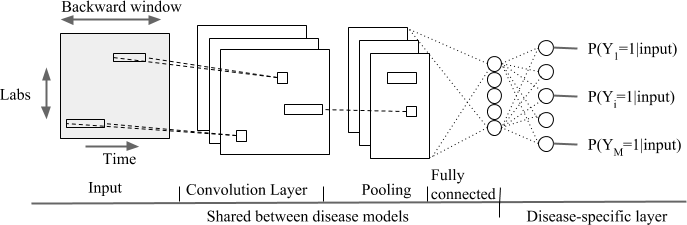
\includegraphics{arch1.png}
\item
  Convolutional neural network over input and time dimension (type =
  mix)

  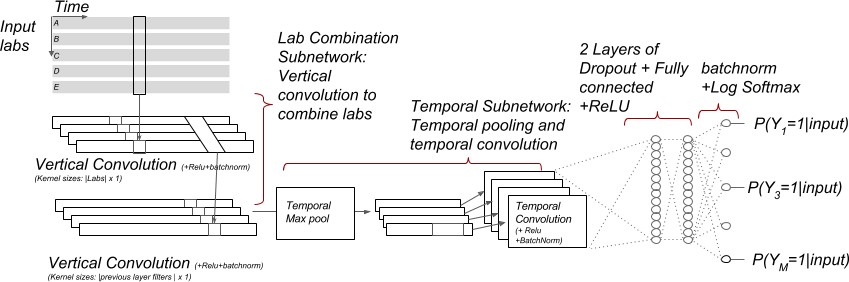
\includegraphics{conv_arch2.png}
\item
  Multi-resolution temporal convolutional neural network (type = multi)

  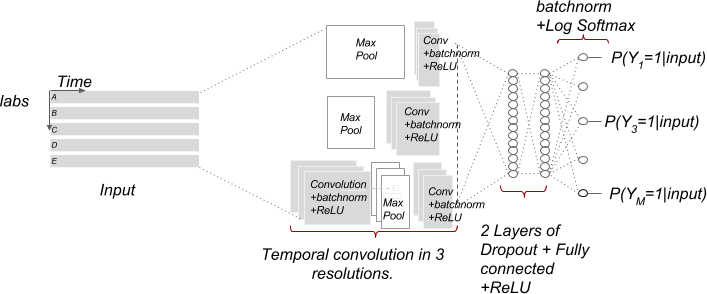
\includegraphics{conv_arch1.png}
\end{enumerate}

Furthermore, we added the following topologies:

\begin{enumerate}
\def\labelenumi{\arabic{enumi})}
\setcounter{enumi}{3}
\item
  CNN with filters with three different parallel kernel sizes (3,4,5)
  and a fully connected layers (type = mlf)

  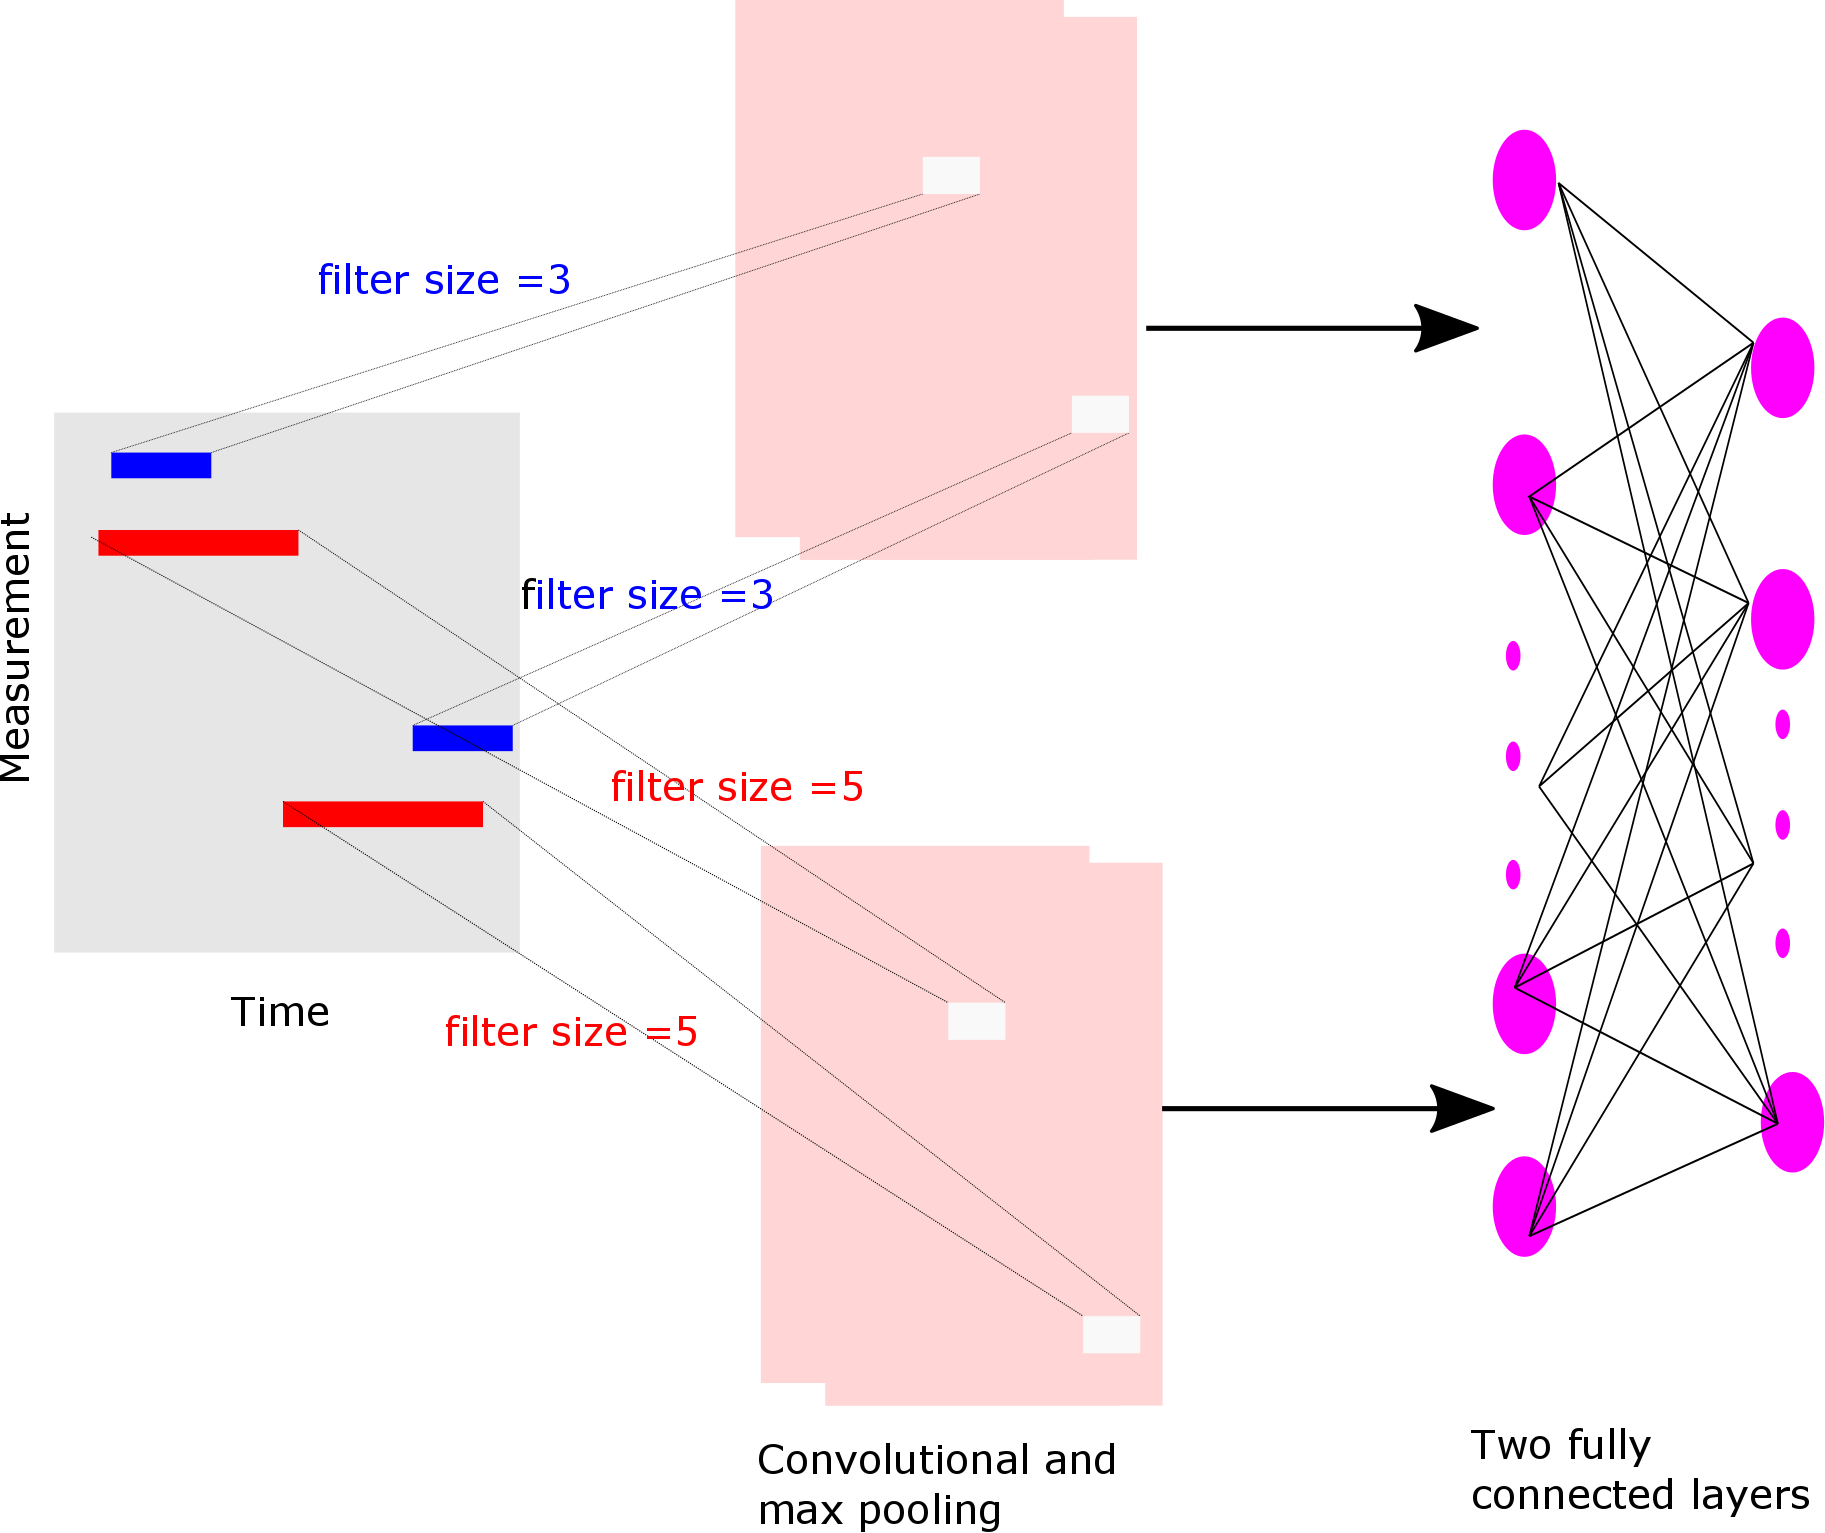
\includegraphics{cnn_mlf2.png}
\item
  LSTM network over the backward window (type = lstm)

  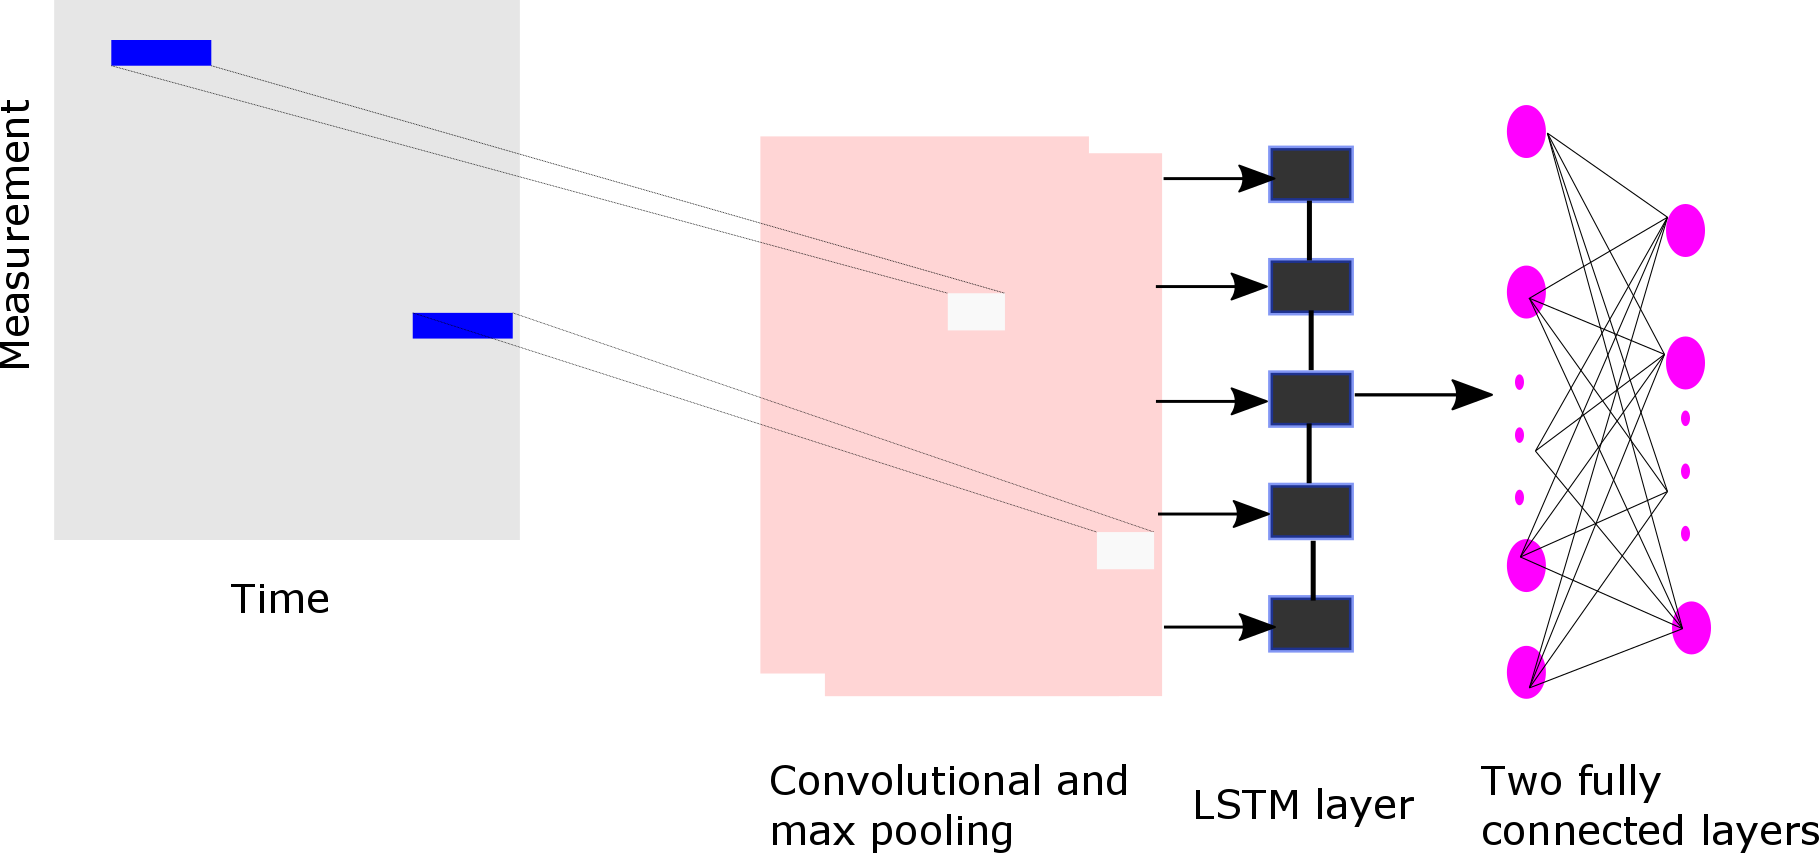
\includegraphics{cnn_lstm.png}
\item
  Residual Learning Network as descripted in:
  \url{https://arxiv.org/abs/1512.03385} (type = resnet)

  This a very big network, see the paper for the topology.
\end{enumerate}

\begin{longtable}[]{@{}ll@{}}
\toprule
\begin{minipage}[b]{0.14\columnwidth}\raggedright\strut
parameter\strut
\end{minipage} & \begin{minipage}[b]{0.35\columnwidth}\raggedright\strut
description\strut
\end{minipage}\tabularnewline
\midrule
\endhead
\begin{minipage}[t]{0.14\columnwidth}\raggedright\strut
nbfilters\strut
\end{minipage} & \begin{minipage}[t]{0.35\columnwidth}\raggedright\strut
The number of convolution filters\strut
\end{minipage}\tabularnewline
\begin{minipage}[t]{0.14\columnwidth}\raggedright\strut
epochs\strut
\end{minipage} & \begin{minipage}[t]{0.35\columnwidth}\raggedright\strut
The number of epochs\strut
\end{minipage}\tabularnewline
\begin{minipage}[t]{0.14\columnwidth}\raggedright\strut
seed\strut
\end{minipage} & \begin{minipage}[t]{0.35\columnwidth}\raggedright\strut
Random seed\strut
\end{minipage}\tabularnewline
\begin{minipage}[t]{0.14\columnwidth}\raggedright\strut
class\_weight\strut
\end{minipage} & \begin{minipage}[t]{0.35\columnwidth}\raggedright\strut
The class weight used for imbalanced data (0: Inverse ratio between
positives and negatives, -1: Focal loss, or number)\strut
\end{minipage}\tabularnewline
\bottomrule
\end{longtable}

\subsection{PyTorch RNN}\label{pytorch-rnn}

The following \textbf{recurrent neural network} models are implemented
in RNNTorch:

\begin{enumerate}
\def\labelenumi{\arabic{enumi})}
\item
  RNN with one LSTM layer fed into one fully connected layer (type =
  RNN)

  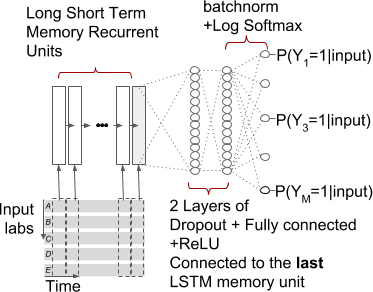
\includegraphics{lstm_last.png}
\item
  RNN with one bidirectional LSTM layer fed into one fully connected
  layer (type = BiRNN)

  This network looks the same as above but then as a bi-directional
  version
\item
  One Gated Recurrent Unit layer fed into one fully connected layers
  (type = GRU)

  This network looks the same as above but then implemented as GRU
\end{enumerate}

The following hyper-parameters can be set for these pyTorch models:

\begin{longtable}[]{@{}ll@{}}
\toprule
\begin{minipage}[b]{0.14\columnwidth}\raggedright\strut
parameter\strut
\end{minipage} & \begin{minipage}[b]{0.35\columnwidth}\raggedright\strut
description\strut
\end{minipage}\tabularnewline
\midrule
\endhead
\begin{minipage}[t]{0.14\columnwidth}\raggedright\strut
hidden\_size\strut
\end{minipage} & \begin{minipage}[t]{0.35\columnwidth}\raggedright\strut
The number of features in hidden state\strut
\end{minipage}\tabularnewline
\begin{minipage}[t]{0.14\columnwidth}\raggedright\strut
epochs\strut
\end{minipage} & \begin{minipage}[t]{0.35\columnwidth}\raggedright\strut
The number of epochs\strut
\end{minipage}\tabularnewline
\begin{minipage}[t]{0.14\columnwidth}\raggedright\strut
seed\strut
\end{minipage} & \begin{minipage}[t]{0.35\columnwidth}\raggedright\strut
Random seed\strut
\end{minipage}\tabularnewline
\begin{minipage}[t]{0.14\columnwidth}\raggedright\strut
class\_weight\strut
\end{minipage} & \begin{minipage}[t]{0.35\columnwidth}\raggedright\strut
The class weight used for imbalanced data (0: Inverse ratio between
positives and negatives, -1: Focal loss, or number)\strut
\end{minipage}\tabularnewline
\bottomrule
\end{longtable}

\subsection{R Keras CNN}\label{r-keras-cnn}

The following temporal architectures were implemented using R Keras:

\begin{enumerate}
\def\labelenumi{\arabic{enumi}.}
\item
  Multi-resolution CovNN model according to
  \url{https://arxiv.org/pdf/1608.00647.pdf} (CovNN.R)

  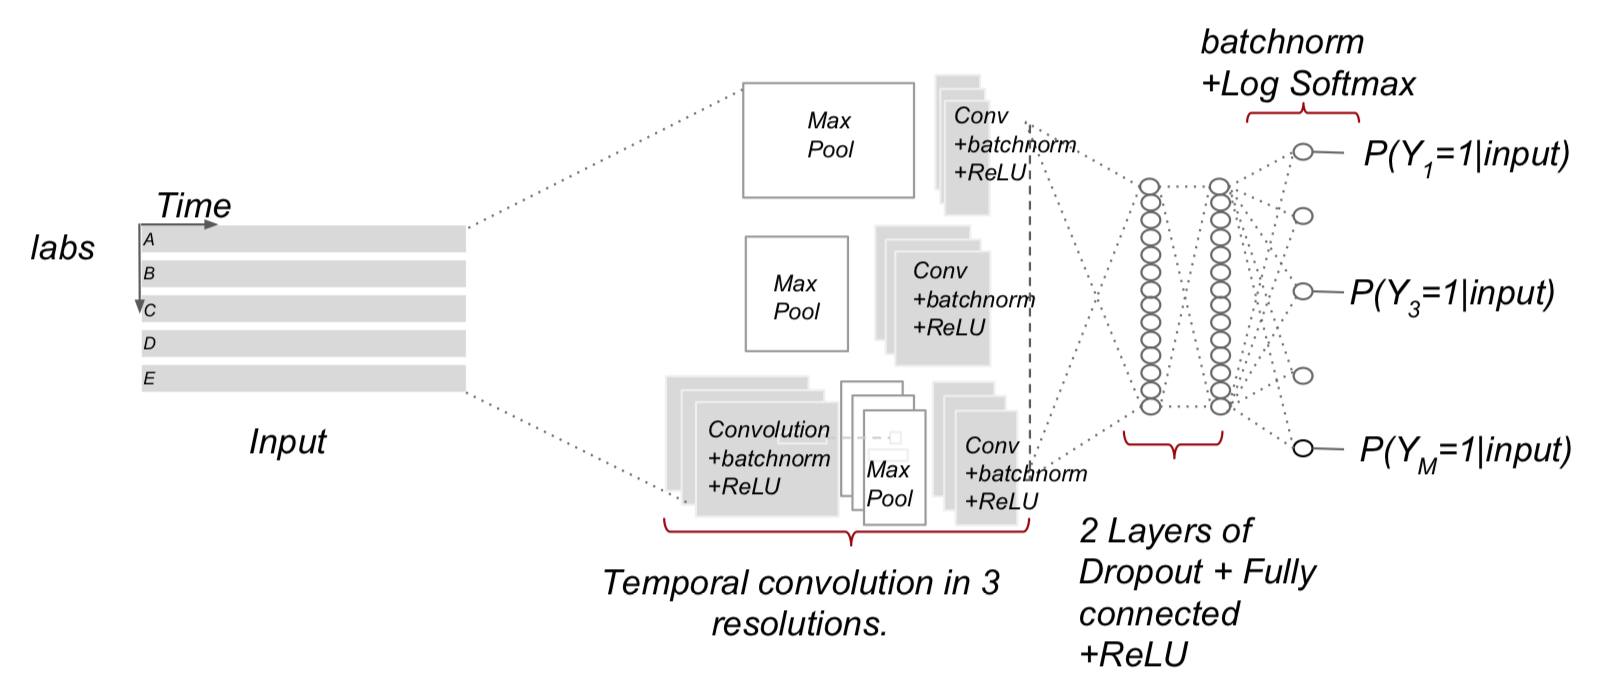
\includegraphics{covcnn.png}
\item
  Convolution accross data and time according to
  \url{https://arxiv.org/pdf/1608.00647.pdf} (CovNN2.R)

  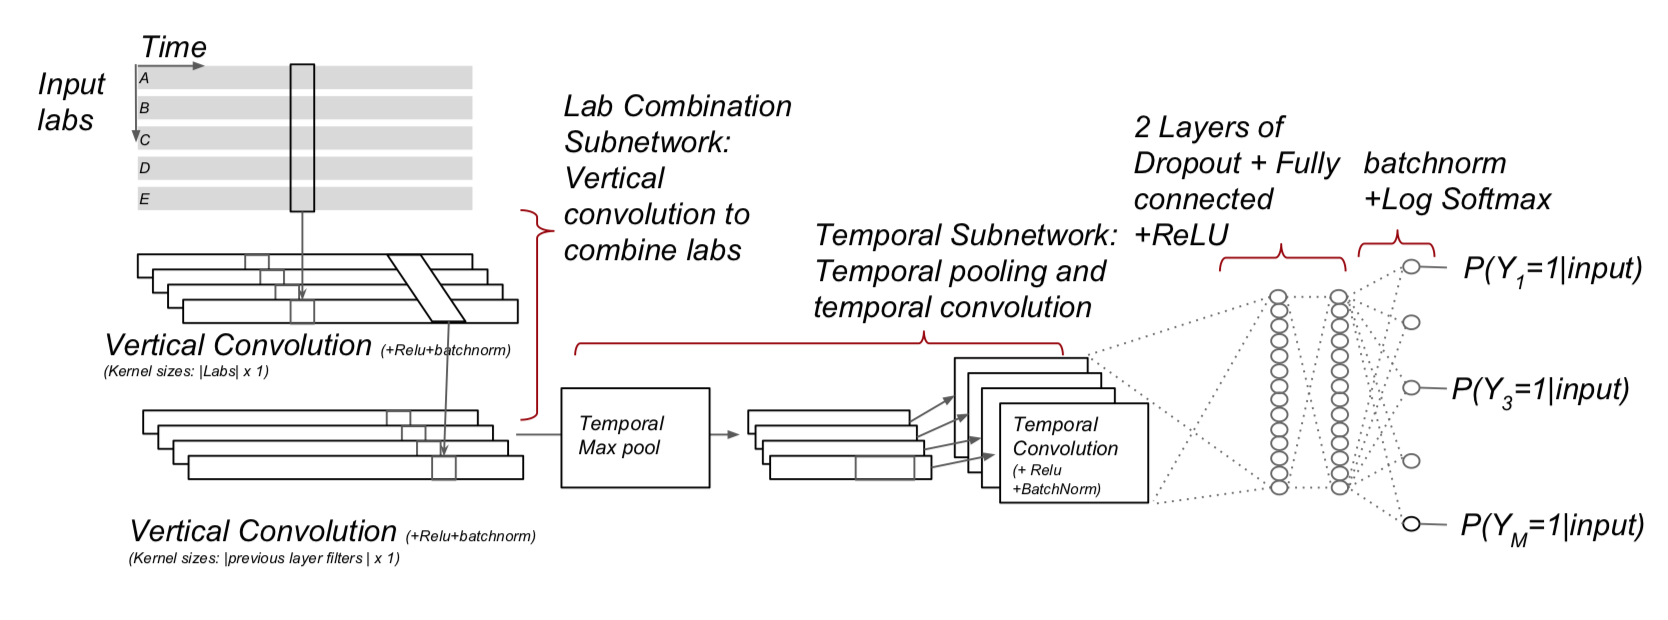
\includegraphics{covcnn2.png}
\item
  Clinically Informing application based on Recurrent Neural Network
  (CIReNN)

  Image to be added.
\end{enumerate}

Table 2: Temporal Deep Learning Models

\begin{longtable}[]{@{}ll@{}}
\toprule
\begin{minipage}[b]{0.12\columnwidth}\raggedright\strut
Model\strut
\end{minipage} & \begin{minipage}[b]{0.82\columnwidth}\raggedright\strut
Hyperparameters\strut
\end{minipage}\tabularnewline
\midrule
\endhead
\begin{minipage}[t]{0.12\columnwidth}\raggedright\strut
CovNN\strut
\end{minipage} & \begin{minipage}[t]{0.82\columnwidth}\raggedright\strut
batchSize (The number of samples to used in each batch during model
training), outcomeWeight (The weight assigned to the outcome), lr (The
learning rate), decay (The decay of the learning rate), dropout
({[}currently not used{]} the dropout rate for regularisation), epochs
(The number of times data is used to train the model, e.g., epoches=1
means data only used once to train), filters (The number of columns
output by each convolution), kernelSize (The number of time dimensions
used for each convolution), loss (The loss function implemented), seed
(The random seed)\strut
\end{minipage}\tabularnewline
\begin{minipage}[t]{0.12\columnwidth}\raggedright\strut
CovNN2\strut
\end{minipage} & \begin{minipage}[t]{0.82\columnwidth}\raggedright\strut
batchSize (The number of samples to used in each batch during model
training), outcomeWeight (The weight assigned to the outcome), lr (The
learning rate), decay (The decay of the learning rate), dropout
({[}currently not used{]} the dropout rate for regularisation), epochs
(The number of times data is used to train the model, e.g., epoches=1
means data only used once to train), filters (The number of columns
output by each convolution), kernelSize (The number of time dimensions
used for each convolution), loss (The loss function implemented), seed
(The random seed)\strut
\end{minipage}\tabularnewline
\begin{minipage}[t]{0.12\columnwidth}\raggedright\strut
CIReNN\strut
\end{minipage} & \begin{minipage}[t]{0.82\columnwidth}\raggedright\strut
units (The number of units of RNN layer - as a list of vectors),
recurrentDropout (The reccurrent dropout rate), layerDropout (The layer
dropout rate), lr (Learning rate), decay (Learning rate decay over each
update), outcomeWeight (The weight of the outcome class in the loss
function), batchSize (The number of data points to use per training
batch), epochs (Number of times to iterate over dataset),
earlyStoppingMinDelta (Minimum change in the monitored quantity to
qualify as an improvement for early stopping, i.e.~an absolute change of
less than min\_delta in loss of validation data, will count as no
improvement), earlyStoppingPatience (Number of epochs with no
improvement after which training will be stopped), seed (Random seed
used by deep learning model)\strut
\end{minipage}\tabularnewline
\bottomrule
\end{longtable}

\subsection{Example}\label{example-1}

We will now show how to use the temporal models by usinng CNNTorch as an
example.

You need to generate a \texttt{population} and \texttt{plpData} object
as described in more detail in
\href{https://github.com/OHDSI/PatientLevelPrediction/blob/master/inst/doc/BuildingPredictiveModels.pdf}{\texttt{BuildingPredictiveModels}
vignette}.

Note that for these algorithms you need to extracted temporal data as
described in the {[}FeatureExtraction vignette{]}
(\url{https://github.com/OHDSI/FeatureExtraction/blob/master/inst/doc/UsingFeatureExtraction.pdf})
as follows:

\begin{Shaded}
\begin{Highlighting}[]
\NormalTok{settings <-}\StringTok{ }\KeywordTok{createTemporalCovariateSettings}\NormalTok{(}\DataTypeTok{useConditionEraStart =} \OtherTok{FALSE}\NormalTok{,}
                                            \DataTypeTok{useConditionEraOverlap =} \OtherTok{FALSE}\NormalTok{,}
                                            \DataTypeTok{useConditionOccurrence =} \OtherTok{FALSE}\NormalTok{,}
                                            \DataTypeTok{useConditionEraGroupStart =} \OtherTok{FALSE}\NormalTok{,}
                                            \DataTypeTok{useConditionEraGroupOverlap =} \OtherTok{FALSE}\NormalTok{,}
                                            \DataTypeTok{useDrugExposure =} \OtherTok{FALSE}\NormalTok{,}
                                            \DataTypeTok{useDrugEraStart =} \OtherTok{FALSE}\NormalTok{,}
                                            \DataTypeTok{useDrugEraOverlap =} \OtherTok{FALSE}\NormalTok{,}
                                            \DataTypeTok{useMeasurement =} \OtherTok{FALSE}\NormalTok{,}
                                            \DataTypeTok{useMeasurementValue =} \OtherTok{TRUE}\NormalTok{,}
                                            \DataTypeTok{useMeasurementRangeGroup =} \OtherTok{FALSE}\NormalTok{,}
                                            \DataTypeTok{useProcedureOccurrence =} \OtherTok{FALSE}\NormalTok{,}
                                            \DataTypeTok{useDeviceExposure =} \OtherTok{FALSE}\NormalTok{,}
                                            \DataTypeTok{useObservation =} \OtherTok{FALSE}\NormalTok{,}
                                            \DataTypeTok{excludedCovariateConceptIds =} \KeywordTok{c}\NormalTok{(}\DecValTok{316866}\NormalTok{),}
                                            \DataTypeTok{addDescendantsToExclude =} \OtherTok{TRUE}\NormalTok{,}
                                            \DataTypeTok{temporalStartDays =} \KeywordTok{seq}\NormalTok{(}\DataTypeTok{from =} \OperatorTok{-}\DecValTok{365}\NormalTok{, }
                                                                    \DataTypeTok{to =} \OperatorTok{-}\DecValTok{1}\NormalTok{, }\DataTypeTok{by =} \DecValTok{12}\NormalTok{), }
                                            \DataTypeTok{temporalEndDays =} \KeywordTok{c}\NormalTok{(}\KeywordTok{seq}\NormalTok{(}\DataTypeTok{from =} \OperatorTok{-}\DecValTok{353}\NormalTok{, }
                                                                    \DataTypeTok{to =} \DecValTok{0}\NormalTok{, }\DataTypeTok{by =} \DecValTok{12}\NormalTok{), }\DecValTok{0}\NormalTok{))}

\NormalTok{plpData <-}\StringTok{ }\KeywordTok{getPlpData}\NormalTok{(}\DataTypeTok{connectionDetails =}\NormalTok{ connectionDetails,}
                        \DataTypeTok{cdmDatabaseSchema =}\NormalTok{ cdmDatabaseSchema,}
                        \DataTypeTok{cohortDatabaseSchema =} \StringTok{"results"}\NormalTok{,}
                        \DataTypeTok{cohortTable =} \StringTok{"cohort"}\NormalTok{,}
                        \DataTypeTok{cohortId =} \DecValTok{11}\NormalTok{,}
                        \DataTypeTok{covariateSettings =}\NormalTok{ settings,}
                        \DataTypeTok{outcomeDatabaseSchema =}\NormalTok{ resultsDatabaseSchema,}
                        \DataTypeTok{outcomeTable =} \StringTok{"cohort"}\NormalTok{,}
                        \DataTypeTok{outcomeIds =} \DecValTok{25}\NormalTok{,}
                        \DataTypeTok{cdmVersion =} \DecValTok{5}\NormalTok{)}
\end{Highlighting}
\end{Shaded}

Each CNN/RNN has several hyper-parameters that can be set as shown in
the Tables above, but for this example we take the defaults.

\begin{Shaded}
\begin{Highlighting}[]
\CommentTok{# specify the the CNN}
\NormalTok{model <-}\StringTok{ }\KeywordTok{setCNNTorch}\NormalTok{(}\DataTypeTok{cnn_type=}\StringTok{'CNN'}\NormalTok{)}
\end{Highlighting}
\end{Shaded}

Run the model training, for example with a testFraction = 0.2 and a
split by person:

\begin{Shaded}
\begin{Highlighting}[]
\NormalTok{results <-}\StringTok{ }\NormalTok{PatientLevelPrediction}\OperatorTok{::}\KeywordTok{runPlp}\NormalTok{(population, plpData, model,}
                                          \DataTypeTok{testSplit=}\StringTok{'person'}\NormalTok{,}
                                          \DataTypeTok{testFraction=}\FloatTok{0.2}\NormalTok{,}
                                          \DataTypeTok{nfold=}\DecValTok{3}\NormalTok{, }
                                          \DataTypeTok{splitSeed=}\DecValTok{1000}\NormalTok{) }
\end{Highlighting}
\end{Shaded}

\section{Apply the trained Deep Learning
model}\label{apply-the-trained-deep-learning-model}

Applying a Deep Learning is identical to the other models in the
package:

\begin{Shaded}
\begin{Highlighting}[]
\CommentTok{# load the trained model}
\NormalTok{plpModel <-}\StringTok{ }\KeywordTok{loadPlpModel}\NormalTok{(}\KeywordTok{getwd}\NormalTok{(), }\StringTok{"\textbackslash{}<model\textbackslash{}>"}\NormalTok{)}

\CommentTok{# load the new plpData (should have the same temporal features!) and create the population}
\NormalTok{plpData <-}\StringTok{ }\KeywordTok{loadPlpData}\NormalTok{(}\KeywordTok{getwd}\NormalTok{(), }\StringTok{"\textbackslash{}<data\textbackslash{}>"}\NormalTok{)}

\NormalTok{populationSettings <-}\StringTok{ }\NormalTok{plpModel}\OperatorTok{$}\NormalTok{populationSettings}
\NormalTok{populationSettings}\OperatorTok{$}\NormalTok{plpData <-}\StringTok{ }\NormalTok{plpData}
\NormalTok{population <-}\StringTok{ }\KeywordTok{do.call}\NormalTok{(createStudyPopulation, populationSettings)  }

\CommentTok{# apply the trained model on the new data}
\NormalTok{validationResults <-}\StringTok{ }\KeywordTok{applyModel}\NormalTok{(population, plpData, plpModel)}
\end{Highlighting}
\end{Shaded}

\section{Adding new architectures}\label{adding-new-architectures}

If you like to add new architectures you have the option to add them
using pyTorch of R Keras.

\subsection{pyTorch}\label{pytorch}

XIAOYONG is working on some text for this.

\subsection{R Keras}\label{r-keras}

JENNA: Add some details

\section{Acknowledgments}\label{acknowledgments}

Considerable work has been dedicated to provide the
\texttt{PatientLevelPrediction} package.

\begin{Shaded}
\begin{Highlighting}[]
\KeywordTok{citation}\NormalTok{(}\StringTok{"PatientLevelPrediction"}\NormalTok{)}
\end{Highlighting}
\end{Shaded}

\begin{verbatim}
## 
##   Jenna Reps, Martijn J. Schuemie, Marc A. Suchard, Patrick B.
##   Ryan and Peter R. Rijnbeek (2018). PatientLevelPrediction:
##   Package for patient level prediction using data in the OMOP
##   Common Data Model. R package version 2.0.5.
## 
## A BibTeX entry for LaTeX users is
## 
##   @Manual{,
##     title = {PatientLevelPrediction: Package for patient level prediction using data in the OMOP
## Common Data Model},
##     author = {Jenna Reps and Martijn J. Schuemie and Marc A. Suchard and Patrick B. Ryan and Peter R. Rijnbeek},
##     year = {2018},
##     note = {R package version 2.0.5},
##   }
\end{verbatim}

\textbf{Please reference this paper if you use the PLP Package in your
work:}

\href{http://dx.doi.org/10.1093/jamia/ocy032}{Reps JM, Schuemie MJ,
Suchard MA, Ryan PB, Rijnbeek PR. Design and implementation of a
standardized framework to generate and evaluate patient-level prediction
models using observational healthcare data. J Am Med Inform Assoc.
2018;25(8):969-975.}


\end{document}
